%----------------------------1----------------------------------
\begin{frame}[t]{Motivación y Definición del Problema.}
    \begin{columns}[c]
        \begin{column}[c]{4cm}
            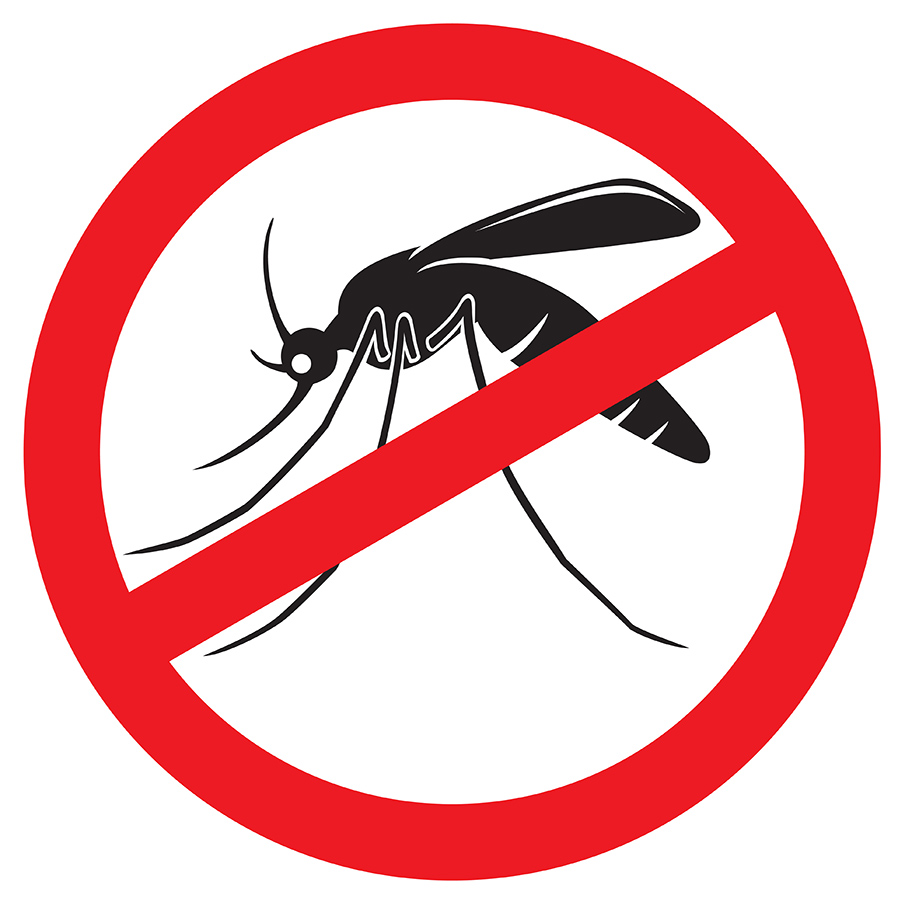
\includegraphics[height=4cm]{./graphics/mosquito.jpg}
        \end{column}

        \begin{column}[c]{6cm} % alternative top-align that's better for graphics
         \begin{itemize}
            \item El Dengue es una enfermedad viral transmitida por el mosquito del Aedes aegypti.
            \item El Aedes aegypti es el principal vector del dengue en América.
            \item Afecta a más de 2,500 millones de personas que viven en zonas de riesgo.
            \item Es considerado un grave problema para la salud pública.
            \end{itemize}
        \end{column}
    \end{columns}
\end{frame}

%----------------------------2----------------------------------

\begin{frame}[t]{Motivación y Definición del Problema.  Criaderos del Aedes aegypti}
    \begin{columns}[c]
        \begin{column}[c]{5cm}
            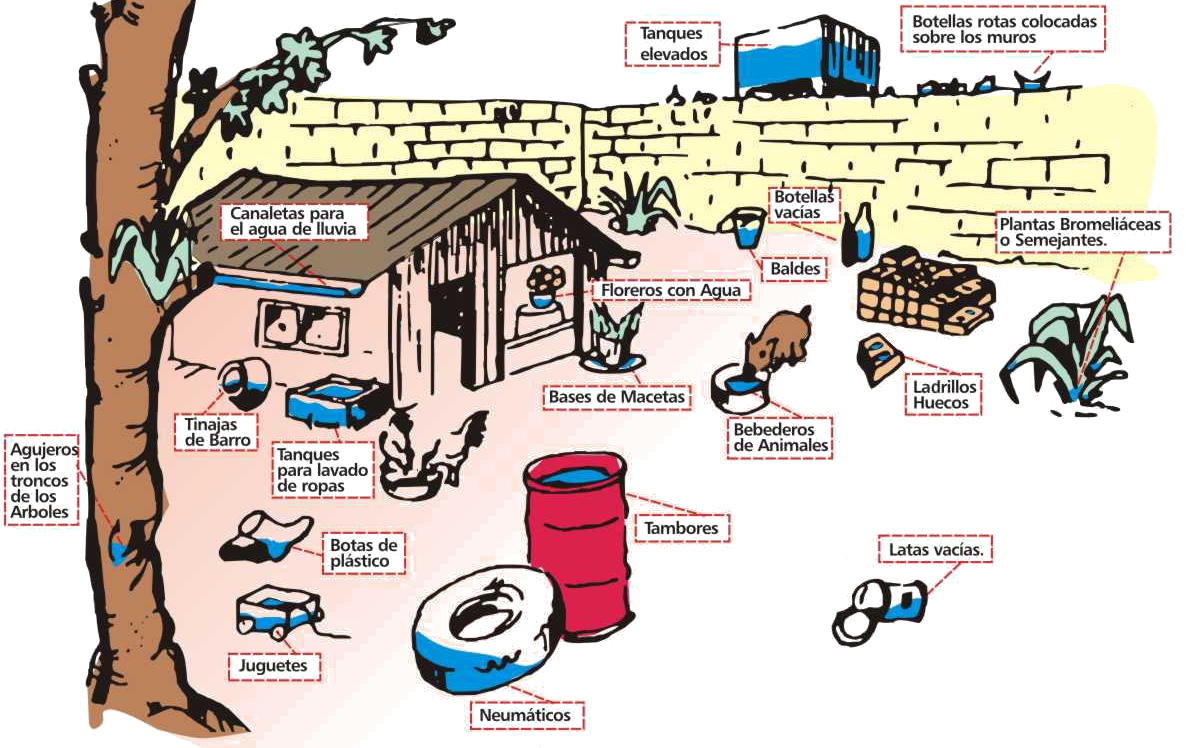
\includegraphics[height=5cm]{../book/capitulo-3/graphics/criaderos-domicilio.png}
        \end{column}

        \begin{column}[c]{5cm}
          \begin{itemize}
          \item Urbanos: baldíos, cementerios, desarmaderos, basurales.

          \item Domésticos: neumáticos, floreros, botellas, bebederos de animales, latas abiertas, prácticamente de cualquier objeto que retenga agua.
          \end{itemize}
    \end{column}
  \end{columns}
\end{frame}

%----------------------------3----------------------------------


%----------------------------4----------------------------------

\begin{frame}[t]{Motivación y Definición del Problema. Dengue en Paraguay.}
  \begin{center}
    \begin{itemize}
    \item El Paraguay desde el año 2009 es considerado un país endémico.

    \item El clima, subtropical, favorece la aparición y desarrollo del dengue.

    \item En las últimas décadas se han observado un crecimiento considerable de las notificaciones de posibles casos de dengue, algunas con derivaciones fatales.

    \item Monitorear el comportamiento el vector con técnicas tradicionales de vigilancia.

    \item Control vectorial para la disminución de las poblaciones de mosquitos.
    \end{itemize}
  \end{center}
\end{frame}

%----------------------------5----------------------------------

\begin{frame}[t]{Motivación y Definición del Problema. Dengue en Paraguay.}
  \begin{center}
  \begin{table}
      \begin{minipage}{\textwidth}
          \begin{center}
          \caption{Histórico de casos de dengue notificados, confirmados y con derivación fatal en Paraguay.}
          \begin{tabular}{l c c r r}
              \hline
              Año & Periodo (inicio / fin) & Notificados & Confirmados & Muertes\\
              \hline
              \hline
              2014 & 29-12-13 / 31-05-14 & 10.541 & 1.052 & 2\\
              2013 & 30-12-12 / 21-12-13 & 153.793 & 131.306 & 70\\
              2012 & 01-01-12 / 22-12-12 & 37.815 & 30.588 & 11\\
              2011 & 03-01-11 / 29-12-11 & 53.397 & 42.264 & 62\\
              2010 & 11-10-09 / 25-12-10 & 21.951 & 13.760 & --$^a$
          \end{tabular}
          \footnotetext[1]{No se encontraron datos sobre muertes en el periodo.}
          \end{center}
      \end{minipage}
  \end{table}
  \end{center}
\end{frame}

%----------------------------6----------------------------------

\begin{frame}[t]{Motivación y Definición del Problema. Vigilancia Entomológica en Paraguay.}

    \begin{itemize}
      \item Para estimar la densidad del vector, la OMS ha recomendado los siguientes indicadores entomológicos : Índice de Casa, Índice de Recipiente e Índice de Breteau.

      \item  Los indices tradicionales, se fundamentan en la detección de la presencia de formas inmaduras del vector dentro de recipientes domésticos.

      \item Son considerados una pobre indicación de la producción de mosquitos adultos.

    \end{itemize}
\end{frame}

%----------------------------7----------------------------------

\begin{frame}[t]{Motivación y Definición del Problema. Vigilancia Entomológica en Paraguay.}
    \begin{itemize}
      \item No reflejan la asociación que existe entre las densidades de mosquitos y tipo de recipientes presentes.

      \item Proporciona poca o nula información de aquellas viviendas en las que existe un mayor riesgo de presencia de mosquitos.

      \item Sólo son recomendados para detectar la calidad de las acciones realizadas por el personal de control larvario.

      \item Existen numerosos métodos e indicadores más prácticos, eficientes y económicos, como larvitrampas y ovitrampas.

    \end{itemize}
\end{frame}

%----------------------------6----------------------------------
\begin{frame}[t]{Motivación y Definición del Problema.}

  \begin{itemize}

    \item Las autoridades sanitarias del Paraguay no cuentan con datos computables, geográficamente, relacionados con a casos reportados, confirmados, sospechosos y fatales de dengue que permitan realizar análisis estadísticos y espaciales.

    \item  Se deben optar por nuevas metodologías que permitan generar información para el análisis sin la necesidad de grandes requerimientos.

    \item Las metodologías de vigilancia entomológica basadas en el uso de larvitrampas y ovitrampas permiten generar información regionalizada sobre el estado y la distribución de la población del vector.

  \end{itemize}
\end{frame}
